\documentclass{article}
\title{\textbf{The Yocto Project - Up and Running}}
\author{}
\date{} 
\UseRawInputEncoding

\usepackage{graphicx}
% Links
\usepackage{hyperref}
\hypersetup{
    colorlinks=true,
    linkcolor=blue,
    filecolor=magenta,      
    urlcolor=cyan,
}
 
\urlstyle{same}

% Code Coloring
\usepackage{xcolor}
\usepackage{listings}
\lstset{
  language=bash,
  basicstyle=\small\sffamily,
  showstringspaces=false
  %numbers=left,
  %numberstyle=\tiny,
  numbersep=3pt,
  %linewidth=13cm,
  frame=tb,
  columns=fullflexible,
  backgroundcolor=\color{yellow!20},
  linewidth=1.4\linewidth,
  xleftmargin=0\linewidth
}


%Box Note
\usepackage{graphicx}
\usepackage{tcolorbox}
\tcbuselibrary{skins}
\usepackage{lipsum}
\definecolor{boxTitle}{HTML}{fff79a}
\definecolor{boxBackground}{HTML}{fffce0}
\definecolor{boxFrame}{HTML}{f1e2b8}

\tcbset{my box/.style={
    enhanced, fonttitle=\bfseries,
    colback=boxBackground, colframe=boxFrame,
    coltitle=black, colbacktitle=boxTitle,
    attach boxed title to top left={xshift=0.3cm,
                                    yshift*=-\tcboxedtitleheight/2},
    boxed title style={
      before upper=\hspace*{0.5cm}, % reserve space for the image
      overlay={
       \node at ([xshift=0.5cm]frame.west)
         {\includegraphics[scale=0.65]{bc-dodecaedre}};
      }
    }
  }
}

\newtcolorbox{mybox}[1][]{my box, #1}

\begin{document}
\textbf{Disclaimer}: This material is a study notes, so for any technical issues please contact me to resolve it periodically.

\begin{minipage}{\textwidth}
    \maketitle
\end{minipage}
\tableofcontents{}
\section{Introducing Yocto}
\subsection{What is the Yocto Project ?}
\textbf{"IT'S NOT AN EMBEDDED LINUX DISTRIBUTION, IT CREATES A CUSTOM ONE FOR YOU. " That's it!.} \\

A Yocto release will have:
\begin{itemize}
    \item Poky, the build system
    \item A build appliance; that is, a VMware image of a host system ready to use Yocto
    \item An Application Development Toolkit (ADT) installer for your host system
    \item And for the different supported platforms:
\begin{itemize}
    \item Prebuilt toolchains
    \item Prebuilt packaged binaries
    \item Prebuilt images
\end{itemize}
\end{itemize}

\subsection{What is Poky ?}
Poky is the Yocto project reference \textbf{build system}, it's originally a branch from OpenEmbedded build system called \textit{bitbake}, and it contains already the metadata of the OE system.

The purpose of Poky is to build the components needed for an embedded Linux product, namely:
\begin{itemize}
    \item A bootloader image
    \item A Linux kernel image
    \item A root filesystem image
    \item Toolchains and software development kits (SDKs) for application development.
\end{itemize}

\subsection{Poky workflow}

\begin{center}
  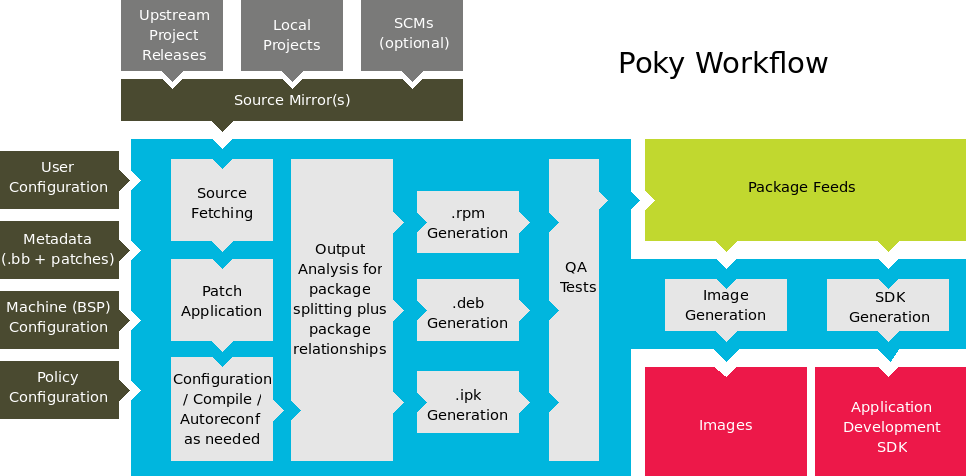
\includegraphics[scale=0.60]{./resources/img/yocto-environment.png}
\end{center}

\begin{enumerate}
  \item \textbf{do\_fetch} - Downloads the source files and additional artifacts needed to construct a specific SW component. The location can be a remote repository or even a local directory. This location is configured using the SRC\_URI variable of a recipe file.
  \item \textbf{do\_unpack} - If the downloaded sources in the previous step are compressed, they are decompressed in this step.
  \item \textbf{do\_patch} - If the source needs to be modified (e.g. due to a known bug), it can be patched in this step using the patch file indicated in the corresponding recipe.
  \item \textbf{do\_configure} - In this phase, the build configuration is defined (e.g. build files are generated, directives are set, …) as a preparation for the coming task.
  \item \textbf{do\_compile} - This is the task where the sources are built and linked to produce deployable binaries.
  \item \textbf{do\_install} - In this task, the produced binaries and any additional files (e.g. images, database files, textual configuration files, …) are grouped together in a folder structure specified by the user (e.g. binaries go to <package>/bin, config. files go to <package>/etc).
  \item \textbf{do\_package} - The packaging operation converts the previously generated folder into a known package format (e.g. .rpm, .deb, ...) to be used by package management applications.
  \\And once all needed components are packaged, the following tasks are executed for the image:
  \item \textbf{do\_rootfs} - Builds a root filesystem that includes the bootloader, the kernel binary, the device tree blob in addition to all packages that need to be deployed in the system.
  \item \textbf{do\_image} - Finally the generated filesystem is converted into a predefined image format (e.g. .sdcard to be deployed onto a SD Card, hard drive image, tarball files, etc…)
\end{enumerate}

\subsection{Building a minimal image using Poky}
So, let's have a quick example on building a full Linux distro using Poky, it's as simple as the following four steps:

\begin{enumerate}
  \item Get Poky
  Just fetch your own branch of Poky, I am using here \textit{morty} branch with Ubuntu 18.04. You need to take care as some distributions of Yocto has already compatibility issues with a certain Liunx images.
  \lstinputlisting[caption=Install Poky]{resources/src/install/1-install-poky}
  
  \item Configure your system
  After getting poky installed just run the \textbf{oe-init-build-env}, and see what happened ?\\
  \lstinputlisting[caption=Config the environment]{resources/src/install/2-init-env-script}
  
  \begin{center}
  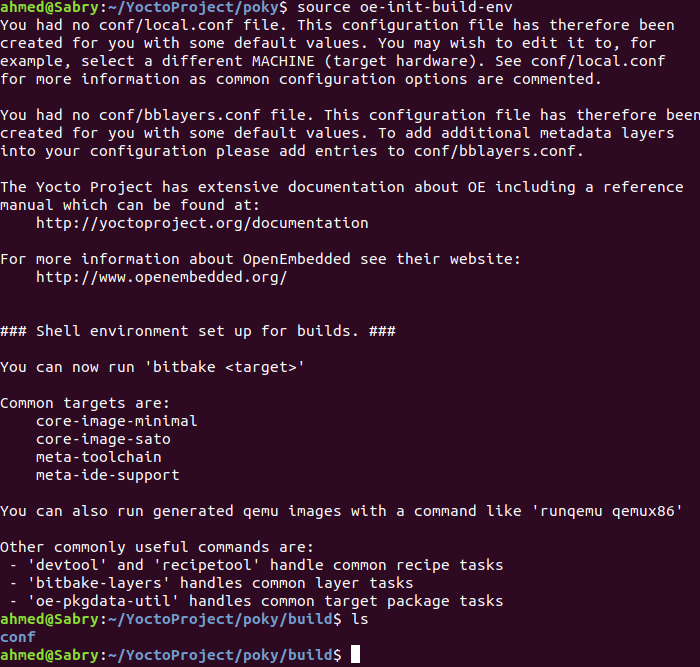
\includegraphics[scale=0.60]{./resources/img/init-env-script.png}
  \end{center}
  it will setup the environment and create a build directory (with conf folder; contains the a build specific conf files, we will take about them later) for us in order to start, and finally here we are in that build directory to \textit{bitbake} our image.
  
\item Build the distro using \textit{bitbake}\\
\lstinputlisting[caption=bitbake a minimal image]{resources/src/install/3-build-minimal-core-image}

Here we are trying to build a minimal Linux distro (something which can boot and run), and as you can see it fetches the stuff and building.


after some do\_complie and do\_package and so on, then you have your own linux image. you can use see the output here \textbf{"build/tmp/deploy/images/qemux86/"}

  \begin{center}
  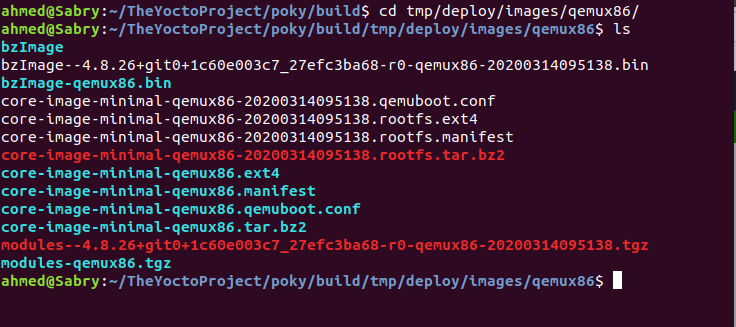
\includegraphics[scale=0.60]{./resources/img/build-output.png}
  \end{center}

as you might noticed that it taken little bit of time for the first time to build. 

\begin{mybox}[title={Note: where to find all the supported images ?}]
  
  Note: you can check all the supported images by the following command:
  \lstinputlisting[caption=Supported Images]{resources/src/install/supported-images}
  
\end{mybox}

  \item Finally, run your first yocto image by using the \textit{qemu} emulator.
    \lstinputlisting[caption=runqemu command to load your image]{resources/src/install/4-runqemu}
  
    \begin{center}
  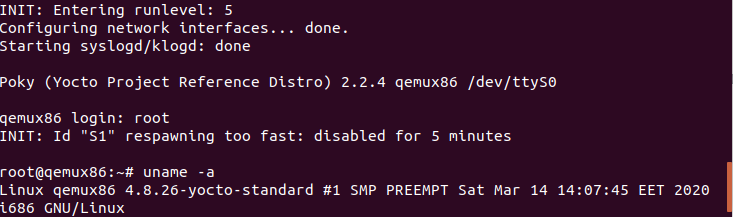
\includegraphics[scale=0.60]{./resources/img/minimal-runqemu.png}
  \end{center}
\end{enumerate}

\subsection{Poky folder structure}
Now after a successful build of our image, let's have a look on \textit{Poky} folder structure.
\lstinputlisting[caption=Yocto folder structure]{resources/src/yocto-structure}

As you can see from the tree-like structure, \textit{Yocto} has the following main folders:
\begin{itemize}
  \item \textbf{bitbake} folder\\
  It contains all the stuff related to the OpenEmbedded (OE) bitbake build system, which is a reference one for Poky.
  \item \textbf{meta-XX} folders (meta, meta-poky, meta-yocto, ...)\\
  Any folder annotated by \textit{meta-}, it will be a layer to contain a certain yocto meta and configuration data. We have here a basic meta layers, and please
  refer to the layers section \nameref{yocto-layers} for more details. \\

  You might noticed that for every layer, there is a at least \textbf{conf} folder which contains a specific layer configuration file.
  \item \textbf{Build} folder:\\
  All the magic while building occurs on this folder, and all your output images and SDKs goes here, and as you might notice that this folder contains:
    \begin{itemize}
      \item \textbf{downloads} folder; which is used while fetching the files before building
      \item \textbf{conf} folder; contains configuration files for the current build, here mainly you will find:
        \begin{itemize}
          \item \textbf{bblayers.conf} file: which contains the configured meta-layers used in the current build
          \item \textbf{local.conf} file: contains some build variables/parameters to customize the build
          
          and both files will be described later.
        \end{itemize}
      \item \textbf{tmp} folder: while building, and all the outputs (SDK, images, ...) will be placed here in this folder.
      \begin{itemize}
        \item \textbf{images} folder: holds all the output images
        \item \textbf{SDKs} folder: holds all the populated SDKs
      \end{itemize}
    \end{itemize}

  \item \textbf{scripts}
  It contains all the python scripts to automate the fetching, build, and packaging. 
  \item \textbf{documentation}
\end{itemize}

Note: You can get all the tree-like structure by using Linux \textit{tree} command, in case you want to explore more.

\subsection{Yocto Project Layers}
\label{yocto-layers}
\begin{center}
  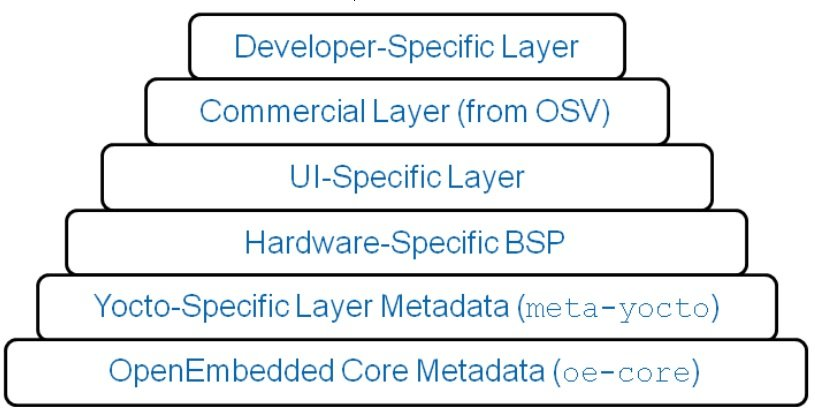
\includegraphics[scale=0.40]{./resources/img/Yocto-Layers.jpeg}
\end{center}

In any Poky version, you will find the following basic layers:
\begin{itemize}
    \item meta: This directory contains the OpenEmbedded-Core metadata which have the base layers of all the build system, for example the basic tasks like \textbf{do\_fetch}, \textbf{do\_compile}, ... are defined in \textbf{base.bbclass} in the OE meta folders.
    \item meta-yocto: This contains Poky's distribution-specific metadata
    \item meta-yocto-bsp: This contains metadata for the reference hardware boards
\end{itemize}

The initial poky build system only supports the following BSP targets, and the virtualized emulators provided by OE-Core, and of course other layers can be included, or defined and customized, you can refer to creating \nameref{simple-custom-layers} section.

\lstinputlisting[caption=Supported virtualized emulators]{resources/src/install/supported-emulators}

\subsection{Basic meta files types}
Yocto has serval files types to support extending your layer:
\begin{itemize}
  \item \textbf{.bbclass files}: Class files contain information that is useful to share between recipes files. An example is the autotools class, which contains common settings for any application that Autotools uses.
  \item \textbf{.bb recipe files}: the files that have the .bb suffix are "recipes" files. In general, a recipe contains information about a single piece of software, and each recipe describes a set of meta info and tasks to do deal with this software unit. 
  \item \textbf{.bbappend files}: You can use a .bbappend file in your layer to make additions or changes to the content of another layer's recipe without having to copy the other layer's recipe into your layer. Your .bbappend file resides in your layer, while the main .bb recipe file to which you are appending Metadata resides in a different layer.
  \item \textbf{.conf files}: The configuration files define various configuration variables that govern the OpenEmbedded build process.
\end{itemize}


\subsection{Basic configuration files}
Finally as an introduction to \textit{Yocto}, we can list some important configuration files which we will deal with a lot in our further sections.

\begin{itemize}
    \item Layers Configuration files:\\ \textbf{build/conf/bblayers.conf} : This file is used to find all the configured layers.\\
    \textbf{meta-xx/conf/layer.conf}: layer specific configuration file.
    \item Build Specific configuration:\\ \textbf{build/conf/local.conf}: This file is used for any other configuration the user may have for the current build
    \item Core configuration files: \\ \textbf{meta/conf/distro/\textless distro \textgreater .conf}: This file is the distribution policy; by default, this is the poky.conf file.\\
    \textbf{meta/conf/bitbake.conf}: this file used to set some default values for overall system, export some core variables, and assign some core configurations.\\
    \textbf{meta/conf/machine/\textless machine\textgreater .conf}: This file is the machine configuration; in our case.\\
\end{itemize}

\section{Writing Layers, Recipes and using the application SDKs}
\subsection{Simple Custom Layer}
\label{simple-custom-layers}
A Yocto layer basically contains set of recipes to describe the workflow for your application building.\\
\begin{center}
  \includegraphics[scale=0.60]{./resources/img/basic-blocks.png}
\end{center}

So in order to write some recipes, it's needed first to create our custom layer, we will create it in two different ways, and we will call it \textbf{my-layer}.

A. You can create a layer automatically by using \textbf{\textit{create-layer}} sub-command, and you need respect the yocto project naming by creating your layer name as follow \textbf{\textit{meta-\textless your-layer-name\textgreater}}, as it helps bitbake while parsing your recipes.
  \lstinputlisting[caption=bitbake-layers create-layer]{resources/src/Layers/CreateLayer00}

By running this command, it will create your layer and append it to the different configuration files in your build system (i.e. append it to bblayers.conf file, and creates layer.conf file).\\

B. Or you can create a layer manually as follow:
\begin{enumerate}
    \item Create a folder for your layer, and you need to respect yocto naming, create it as \textit{meta-mylayer}
    \lstinputlisting[caption=Create the layer folder]{resources/src/Layers/CreateLayer01}
    
    \item Create a layer config file, in \textbf{"/poky/meta-mylayer/conf/layer.conf"}
    
    \lstinputlisting[caption=add layer config file]{resources/src/Layers/CreateLayer-02-CreateLayerConfigFile}
    \item Enabling your layer by adding it to your image, you can do that either by using \textit{bitbake-layers add-layer} command or by adding it manually to \textbf{bblayers.conf} file 
    
    \lstinputlisting[caption=include your layer]{resources/src/Layers/CreateLayer03-EnableYourLayer}
    
    \begin{center}
  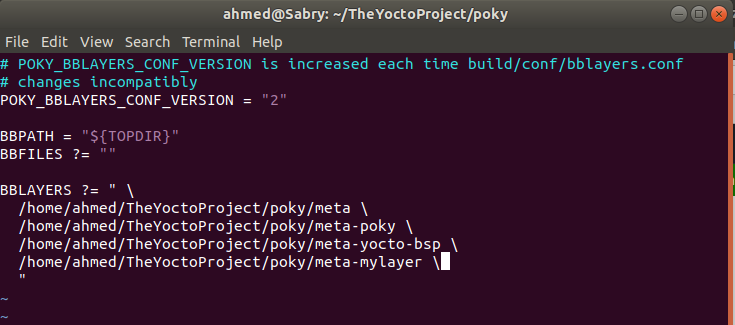
\includegraphics[scale=0.60]{./resources/img/append-to-bblayer.confFile.png}
\end{center}
\end{enumerate}

\begin{mybox}[title={Note: Yocto meta-layer index site ?}]
\begin{itemize}
    \item Before creating a specific layer, you need to look at the \href{https://layers.openembedded.org/layerindex/branch/master/layers/}{Yocto metadata Index site} for already created layers, it might fit your needs.
    \item if you would like your layer to be global at the index, fill the application of yocto project compatible \href{https://www.yoctoproject.org/ecosystem/branding/compatible-registration/}{here}
\end{itemize}  
\end{mybox}


Finally let's create our own image; you need to create \textbf{recipes/images} as follow, then we will use a pre-existing defined image from \textbf{\textit{meta}} layer (\textbf{core-image-minimal.bb}), then customize it to include the "mc" application. 

    \lstinputlisting[caption=create an image recipe]{resources/src/Layers/CreateCustomImage}
    
    \begin{center}
  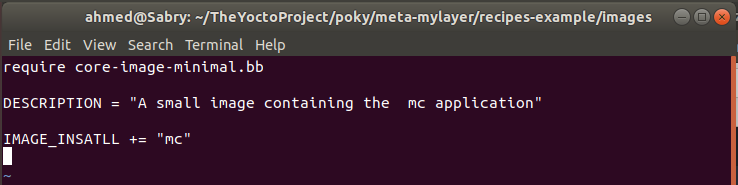
\includegraphics[scale=0.60]{./resources/img/add-mc-to-install.png}
  \end{center}
  
    \lstinputlisting[caption=building our custom image]{resources/src/Layers/bitbake_example-image}
    
    in order to overcome this error, we need to refer to the absolute path of the \textbf{core-image-minimal.bb}.
    \begin{center}
  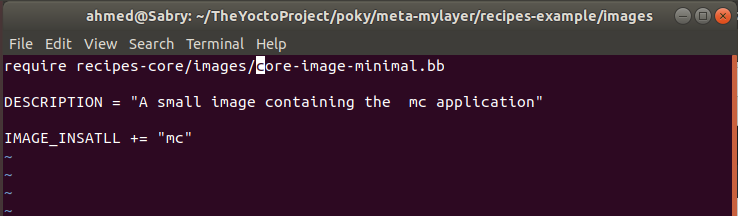
\includegraphics[scale=0.60]{./resources/img/error-cantfindrecipe-core-minimal-solution.png}
  \end{center}
  
  then here we go, a minimal image with "mc" command based on our new custom layer.
  
\begin{center}
  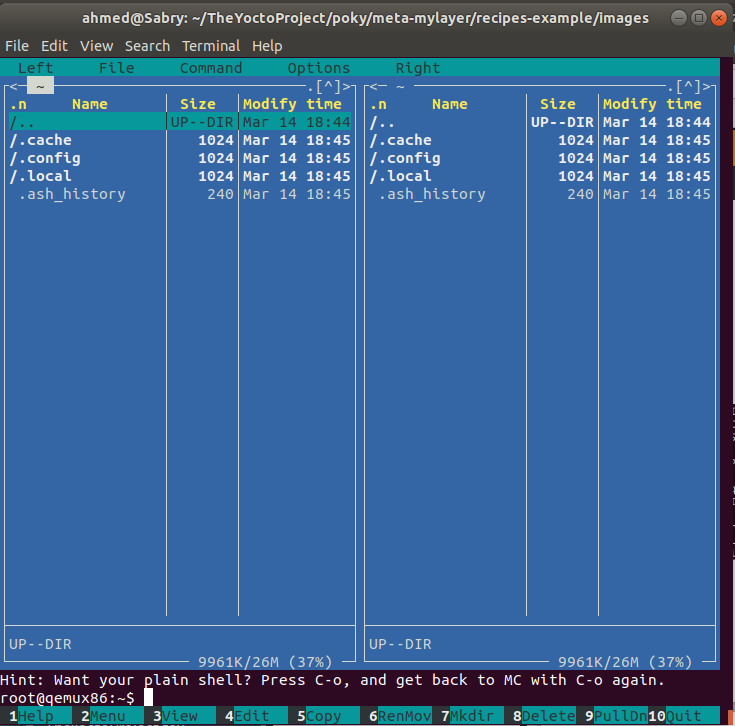
\includegraphics[scale=0.50]{./resources/img/image-with-mc-command.png}
\end{center}

\subsection{Writing recipes}  
\subsubsection{Writing recipes manually}
Now it's time to create a new recipe to build our "Hello Yocto!" program and add it to the bin folder of our custom image.
  
in the folder \textbf{ meta-mylayer/recipes-example} create an \textbf{example} folder and inside it you need to create \textbf{hello-0.1.bb} recipe and hello.c file.

\lstinputlisting[caption=hello.c file]{resources/src/recipes/hello.c}

and the recipe file as follow:

\lstinputlisting[caption=hello-0.1 recipe]{resources/src/recipes/hello-0.1.bb}

\lstinputlisting[caption=building using bitbake]{resources/src/recipes/build}
  
To add the output of this recipe to our custom image, you need to add the your recipe to your conf/local.conf file in your Yocto build directory:

\textbf{IMAGE\_INSTALL\_append = " hello-0.1"}\\

or you can append it to the images file of your layer in \textbf{meta-mylayer/recipes-example/images/example-image.bb}

\begin{mybox}[title={Note: Recipes programming commands}]
  A normal bitbake recipes commands are a mix of python and bash commands!  
\end{mybox}

\begin{center}
  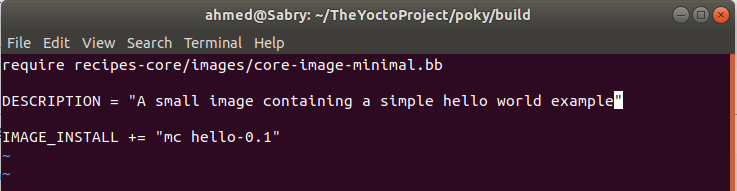
\includegraphics[scale=0.60]{./resources/img/add-hello-to-image-recipe.png}
\end{center}

after booting-up your custom image,  the output is here !
\begin{center}
  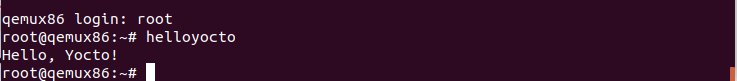
\includegraphics[scale=0.60]{./resources/img/hello-yocto-recipe.png}
\end{center}

\subsubsection{Using Devtool to automatically create recipes}
\textbf{devtool} is an automated recipe creator, build and deploy tool. simply you can add your new packages or modules to your OS image as a new recipes and setup your environment automatically. and the following are devtool simple commands to deal with the recipes:

\begin{itemize}
\item devtool add: Assists in adding new software to be built.
\item devtool modify: Sets up an environment to enable you to modify the source of an existing component.
\item devtool upgrade: Updates an existing recipe so that you can build it for an updated set of source files.
\end{itemize}

\textbf{Types of projects currently supported by devtool:}
\label{devtool-supported-projects}
\begin{enumerate}
  \item autotools (autoconf, and autotools)
  \item cmake
  \item qmake
  \item plain makefile
  \item Binary Packages
  \item out-of-tree kernel module
  \item Node.js Module.
  \item Python modules that use setuptools or distutils.
\end{enumerate}

\textbf{Let's have an example to automatically create our recipes using devtool: }\\
Prerequisites: Github repo containing our code and our build environment, here we are using \textbf{cmake}, devtool will read the \textbf{CMakeFile.txt} and create our recipe accordingly, and you need to notice that devtool can work with different build environments as mentioned in \nameref{devtool-supported-projects}.\\
\begin{center}
  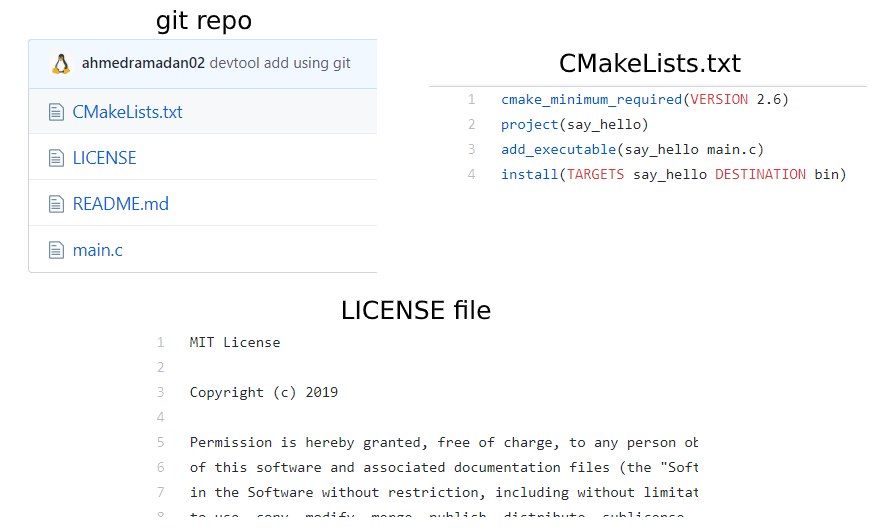
\includegraphics[scale=0.4]{./resources/img/devtool-git-repo.png}
\end{center}

\begin{enumerate}
  \item Use devtool add to create your recipe from the github repo.\\
  \lstinputlisting[caption=Devtool add]{resources/src/devtool/devtool-add}
  
  The recipe is created and you might noticed that by using the devtool, all the stuff is going to be in \textbf{"/build/workspace/recipes"} folder. also devtool will add this \textbf{workspace} folder to the \textbf{bblayers.conf} automatically.
  \begin{center}
    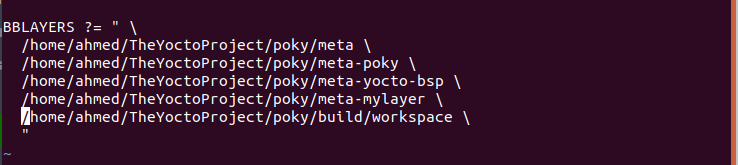
\includegraphics[scale=0.60]{./resources/img/devtool-bblayers.png}
  \end{center}

  and the output recipes is created as follow, by inheriting the \textbf{cmake} and adding our MIT license:
  \begin{center}
    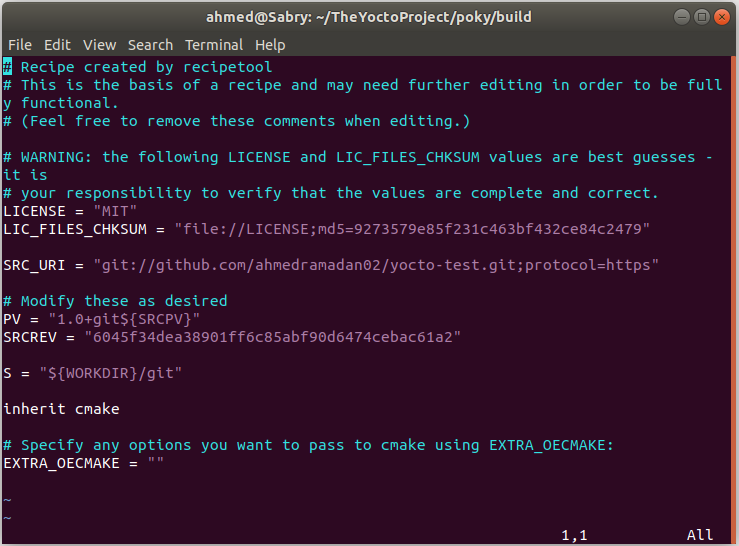
\includegraphics[scale=0.60]{./resources/img/devtool-edit-recipe.png}
  \end{center}
  

  \item use the devtool edit command to make some edits before bitbaking our recipe.
  \lstinputlisting[caption=Devtool edit]{resources/src/devtool/devtool-edit}

  \item then we can use devtool to build our recipe\\
  \lstinputlisting[caption=Devtool build a certain recipe]{resources/src/devtool/devtool-build-recipe}

  You need add the recipe first to your \textbf{local.conf} file, and then build the image.
  \begin{center}
    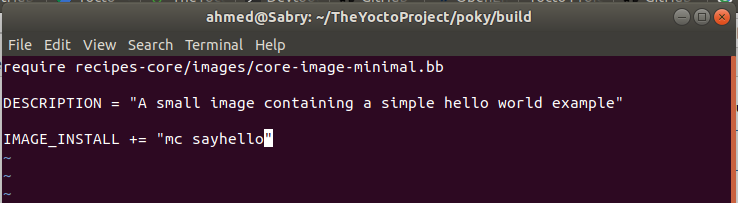
\includegraphics[scale=0.60]{./resources/img/devtool-deploy01.png}
  \end{center}

  \lstinputlisting[caption=Devtool build the image]{resources/src/devtool/devtool-build-image}
  
  \item deploy your recipe to your image (optional if you added the recipe already to \textbf{local.conf} file)\\
  after bitbaking "sayhello", you can directly transfer it to our image by using \textbf{bitbake deploy} command. and in order to do so, your image should be runninng as \textbf{devtool deploy} command uses the same way as \textbf{scp} command.
  \lstinputlisting[caption=Devtool deploy-image]{resources/src/devtool/devtool-deploy}

  Here we go, the following is the deployed binary, before and after using the \textbf{devtool deploy} command:
  \begin{center}
    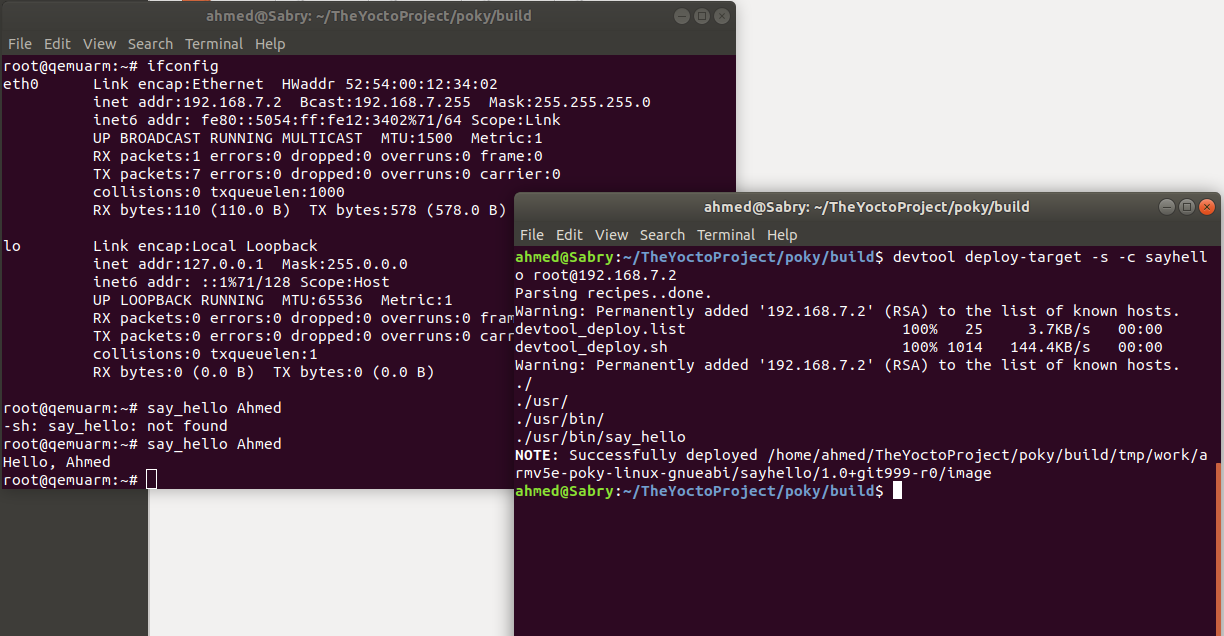
\includegraphics[scale=0.40]{./resources/img/devtool-deploy-target01.png}
  \end{center}

  Note:
  In order to use the \textbf{devtool deploy} feature, you need to edit your \textbf{build/conf/local.conf} file to add the ssh server feature (e.g. openssh, or ssh-server-dropbear) to your image and bitbake it again.

  \begin{center}
    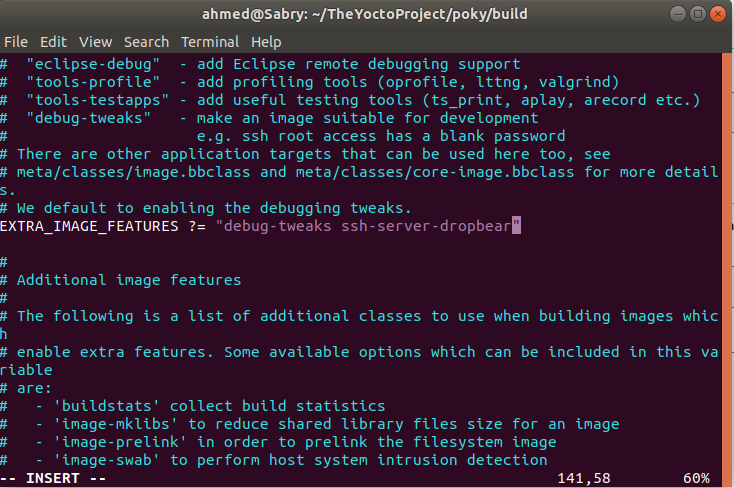
\includegraphics[scale=0.6]{./resources/img/image_features-add-ssh-dropbear.png}
  \end{center}
\end{enumerate}
  

\subsection{Dependencies}
There are couple of run-time and compile time dependencies that you can specify in a recipe. for the compile time, you let bitbake realize that and build it with your binary at the compile time. and the run-time dependencies is used at the run time to make your software able to run.

You can add dependencies using the depend variable as the below example:

\subsection{Package Splitting}
Beside the package we build, we can use bitbake to install other packages which can be installed upon request.

\subsection{Preparing the SDKs for your application development}
In order to develop an applications for your target, you might use one of the following way to achieve that:

\begin{enumerate}
  \item Native Development
  In native development we compile directly on the target machine by a native tool-chain, which means if we compiling for x86, the we use compiler natively and compile on our x86 target. as a summary the target is the host machine for the tool chain.
  In order to include the tool chain to our image, we need to edit \textbf{local.conf} file to add a new \textbf{"tools-sdk"} as a new feature.
  
  \begin{center}
    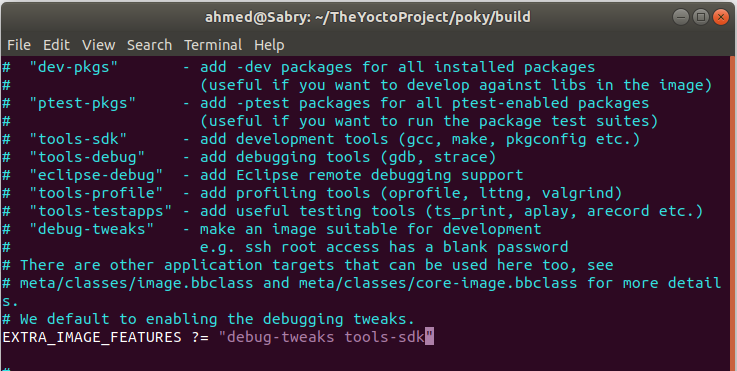
\includegraphics[scale=0.6]{./resources/img/adding-tools-sdk-to-coreminimal.png}
  \end{center}
  after we bitbake our image, here we have our core-image-minimal with only "5.1 MB".

  \begin{center}
    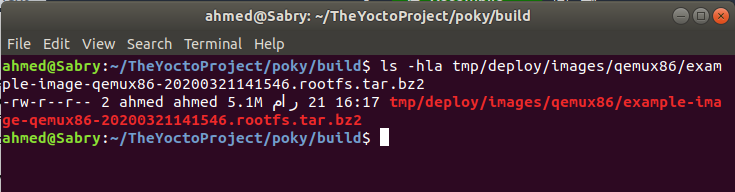
\includegraphics[scale=0.6]{./resources/img/core-minimal-size-without-sdk.png}
  \end{center}

  and now after including a basic tools, we have our image with "70 MB" size!, which 14 times the original size.
  \begin{center}
    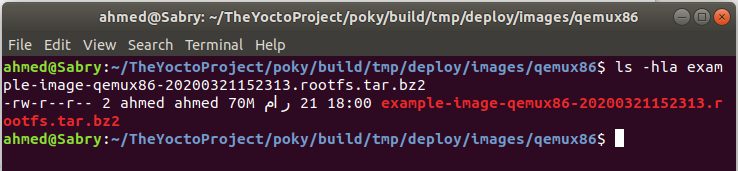
\includegraphics[scale=0.6]{./resources/img/core-minimal-size-with-sdk.png}
  \end{center}

  Unfortunately, as you see the size of the our image is very big as we included the complete tool chain into it, this sounds okay if we will use our image on an efficient PC, but in the world of embedded systems this is not accepted at all, as the footprint of the image should be less, and the processing power needed for compilation might not be that efficient. so we need to introduce the other way which using a cross-compiler.

  \item Cross-Development using a cross-complier on a host system.\\
  simply you develop and build on powerful "host" machine for your target machine, then send the output to be executed on the "target" machine.
  \begin{center}
    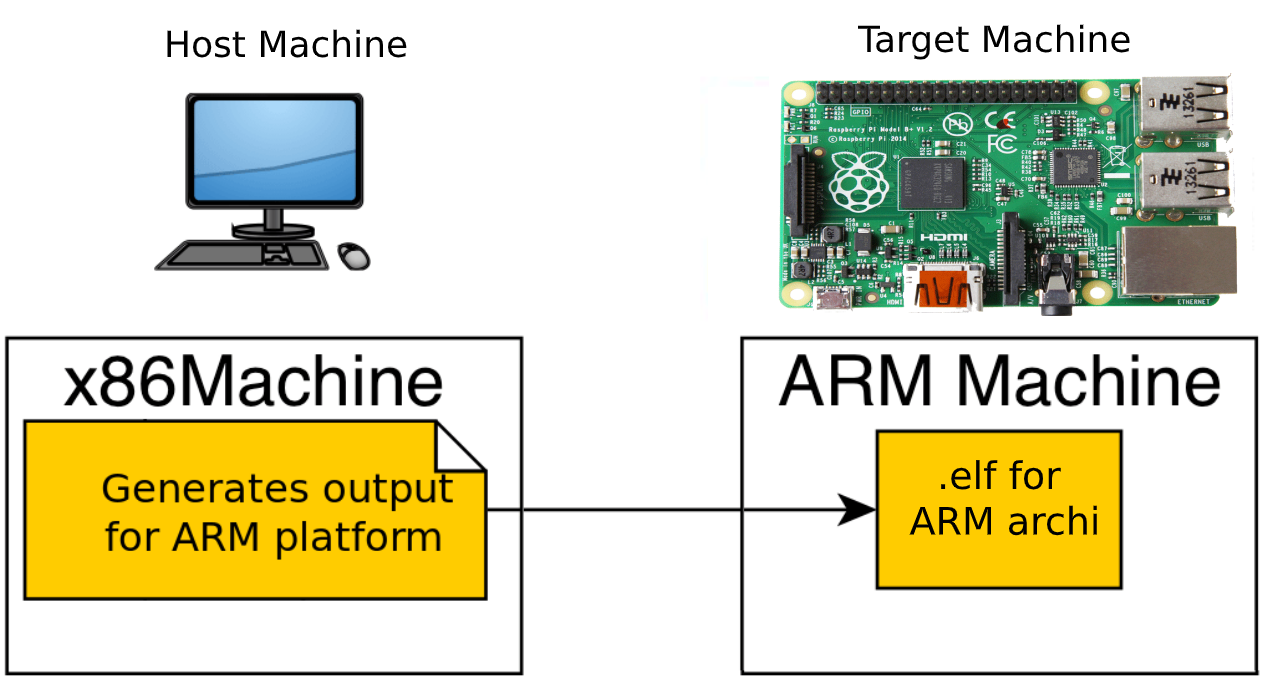
\includegraphics[scale=0.3]{./resources/img/cross-compile.png}
  \end{center}

  first let's change our machine to ARM in order to generate an SDK for it. we can do this by editing \textbf{local.conf} file to comment \textbf{"MACHINE ??= qemux86"} and uncomment \textbf{"MACHINE ?= qemuarm"}.
  \begin{center}
    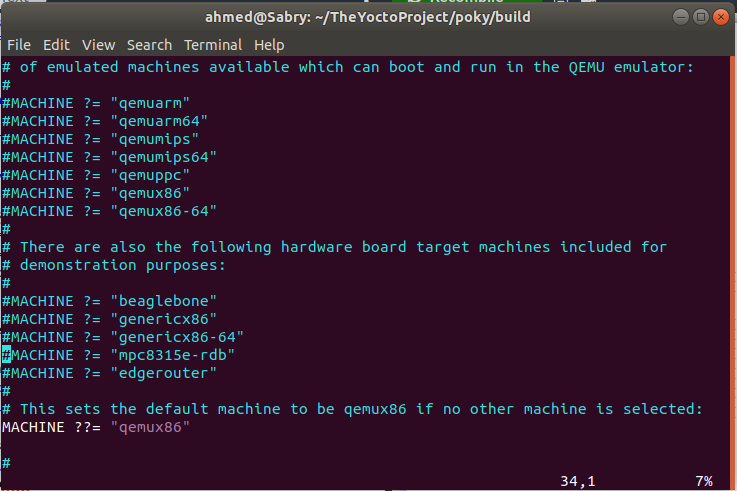
\includegraphics[scale=0.6]{./resources/img/qemuarm.png}
  \end{center}

  then let's get our ARM based cross-sdk:
  \begin{enumerate}
    \item Use populate\_sdk command to fetch your SDK\\
    You can simply use the following command in order to have an SDK for your target
    \lstinputlisting[caption=building using bitbake]{resources/src/sdk/std_sdk}
    
    and it's simply calls the do\_populate task in order to fetch the SDK for your target. and the output is an archived SDK in the following path \textbf{"build/tmp/deploy/sdk"}:
    \lstinputlisting[caption=STD SDK location]{resources/src/sdk/std_sdk_info}

    \item Extract your SDK\\
    I will extract my STD SDK in "~/TheYoctoProject/std\_sdk", and I will do that by calling the compressed SDK ".sh" file in "/build/tmp/deploy/sdk"
    \lstinputlisting[caption=Extract the SDK]{resources/src/sdk/std_sdk_extract}
    
    \begin{center}
      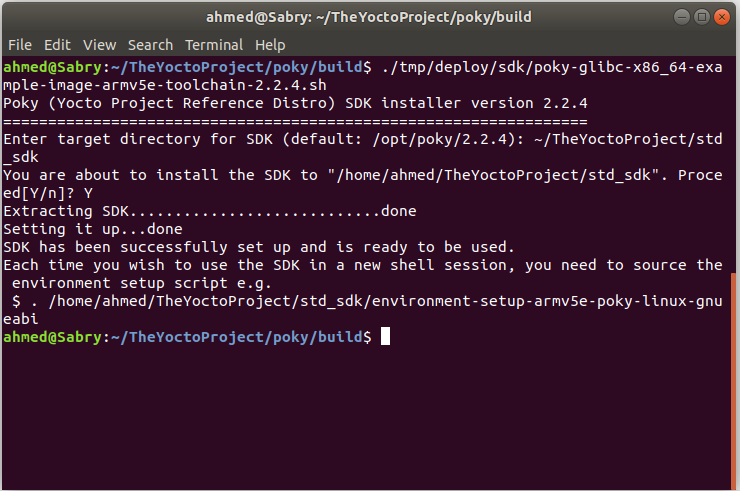
\includegraphics[scale=0.6]{./resources/img/std_sdk_extract.png}
    \end{center}

    \item Compile for your target\\
    In order to compile for your target, you need to execute the output script \textbf{"environment-setup-armv5e-poky-linux-gnueabi"} in the extracted SDK. this script will setup the environmental variables for the cross-compilation for you.

    \lstinputlisting[caption=Setup the environmental variables]{resources/src/sdk/std_sdk_run}
    then simply, use \textbf{cmake} to compile for your target:

    \lstinputlisting[caption=Compile using the cross complier]{resources/src/sdk/std_sdk_complie}

    \item Try on the target machine\\
    Finally, we need to execute the output on our target, We will use the \textbf{scp} command in order to transfer the binary file to the target.
    \lstinputlisting[caption=scp command to transfer our binary to the image]{resources/src/sdk/std_sdk_scp}

    and finally, our application is working as expected
    \begin{center}
      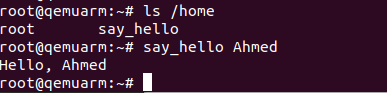
\includegraphics[scale=0.6]{./resources/img/std_sdk_scp.png}
    \end{center}

    Notes: 
    \begin{enumerate}
      \item In order to use scp command, you need to configure your image to include an ssh server, then you need to edit the \textbf{local.conf} file to include openssh for example. here I am using "".
      \begin{center}
        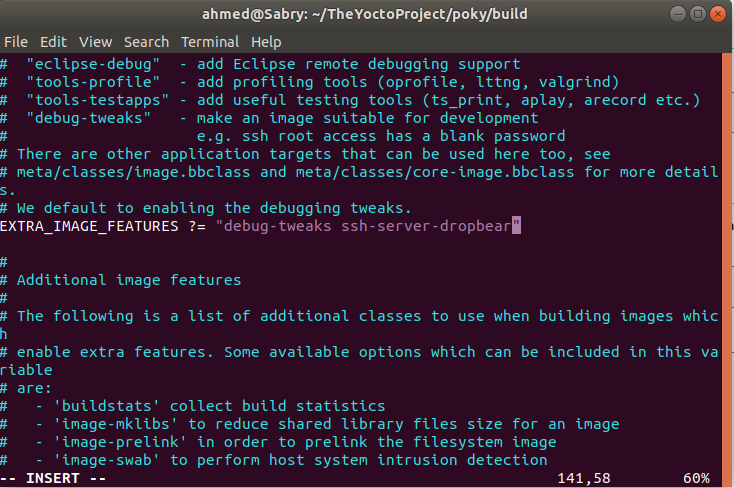
\includegraphics[scale=0.6]{./resources/img/image_features-add-ssh-dropbear.png}
      \end{center}

      \item You might use devtool deploy command to directly build and deploy to your target as we covered previously.
    \end{enumerate}

  \end{enumerate}

  \subsubsection{Types of SDKs}
  With \textit{Yocto}, there are different types of SDKs:
  \begin{enumerate}
      \item Standard SDK
        Which contains just the needed tool chains to build your application. as we already covered how to fetch it and used it in the previous section.

      \item Extensible SDK
      It extends the STD SDK to add more feature mainly you can say that it include a yocto image to create, edit recipes.
      \begin{itemize}
        \item Contains the Toolchain
        \item Contains everything to re-create images, also it have the devtool command.
      \end{itemize}
      
        You can fetch the EXT SDK by executing the following command:
        \lstinputlisting[caption=populating the EXT SDk]{resources/src/sdk/ext_sdk}

        and you might notice the difference in size between the STD SDK and the EXT SDK!.
        \lstinputlisting[caption=STD SDK size V.s. EXT SDK Size]{resources/src/sdk/sizeof-ext-vs-std}
  \end{enumerate}

\end{enumerate}

\section{Packaging}


\section{building an image for Raspberry Pi Board}
In the following section we will make a simple steps to have a ready to run image for raspberry pi. also we will be using it's cross-toolchain in order to build our pi applications, then to see the different ways to deploy the resultant image to run on our pi.

And as you will see that we kind of repeating the previous sections to have this image. 

\begin{enumerate}
    \item Downloading the raspberry pi meta layer.
    \lstinputlisting[caption=clone rpi meta-layer]{resources/src/pi/1-get-pi-meta}
    
    Note: Here I am using \textit{Poky} with \textbf{morty} version, so make sure to branch the raspberry pi for the \textbf{morty} version (morty branch of rpi meta-layer) as well to avoid compatibility issue. otherwise I got some issues.
  

    \item configuring the environment
    \begin{itemize}
        \item Edit the bblayer.conf file to include the pi layer
        \lstinputlisting[caption=add pi meta-layer to bblayer.conf]{resources/src/pi/4-edit-bblayer.bb-file}
        
        \begin{center}
          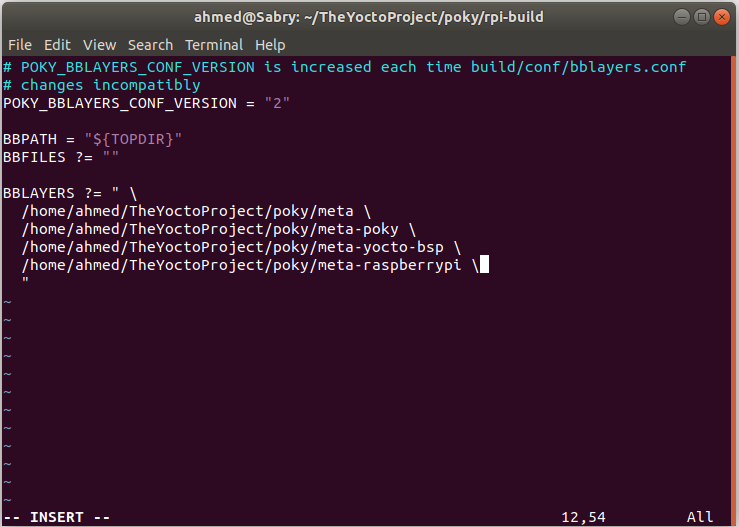
\includegraphics[scale=0.60]{./resources/img/bblayers.conf-add-rpi-layer.png}
        \end{center}

        \item Call the init build script to create a build directory for pi.
        \lstinputlisting[caption=call the init script for our new rpi build]{resources/src/pi/2-call-init-build-script}
        
        We passed \textbf{rpi\_build} to the \textbf{oe-init-build-env} script, so our build folder will be specified as \textbf{rpi\_build} instead of \textbf{build}.

        \item Edit the local.conf file in our new build to build for our new machine "raspberrypi"\\
        before editing \textbf{local.conf}, we need to check all the supported machines in our new raspberry pi meta-layer as follow:
        \lstinputlisting[caption=check all the supported machines in rpi metalayer]{resources/src/pi/3-all-machines}

        And as we are working on raspberry 1 model B, then we will change the \textbf{MACHINE="raspberrypi"} varaible in \textbf{local.conf}.
        \lstinputlisting[caption=choose our new machine from local.conf]{resources/src/pi/3-edit-local.conf}

        \begin{center}
          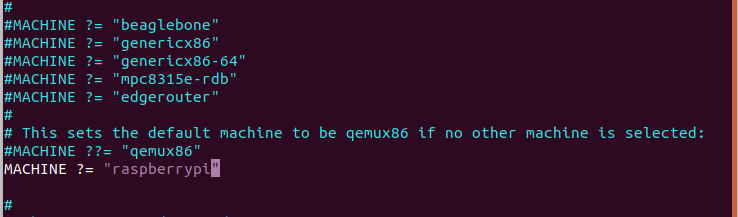
\includegraphics[scale=0.60]{./resources/img/local.conf-rpi.png}
        \end{center}

        \begin{mybox}[title={Note: Note: All mahines with the BCM SoC number: ?}]  
          raspberrypi (BCM2835)\\
            raspberrypi0 (BCM2835)\\
            raspberrypi0-wifi (BCM2835)\\
            raspberrypi2 (BCM2836 or BCM2837 v1.2+)\\
            raspberrypi3 (BCM2837)\\
            raspberrypi4 (BCM2838)\\
            raspberrypi-cm (BCM2835)\\
            raspberrypi-cm3 (BCM2837)\\
        \end{mybox}

    \end{itemize}
    
    
    \item Bitbake the image\\
    \lstinputlisting[caption=bitbake the raspberry pi]{resources/src/pi/6-bitbake-build-pi}

    And the output image will be in the \textbf{"rpi-build/tmp/images/raspberrypi"} folder.
    \begin{center}
      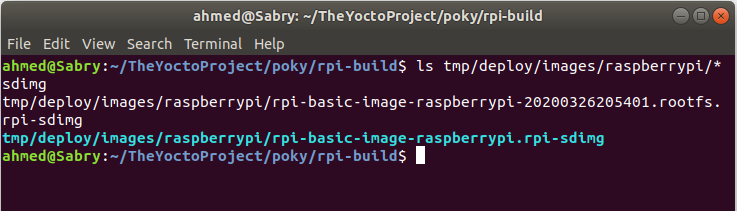
\includegraphics[scale=0.60]{./resources/img/rpi-output-image.png}
    \end{center}
    

    \item Deploy to our SD card
    First look on which sdx the sd card has been mounted in order to use the \textbf{dd} command with it:
    \lstinputlisting[caption=Check SD card mount point]{resources/src/pi/7-1-look-which-dev-file}
        
    FYI: you can use \textbf{lsblk} command also:
    \lstinputlisting[caption=Check SD card mount point]{resources/src/pi/7-2-lsblk}

    Here we use the \textbf{dd} command in order to partition our SD card for our image.
    \lstinputlisting[caption=building using bitbake]{resources/src/pi/7-send-to-sd-card}
    
    then you can check your \textbf{dd} command output as follow:
    \lstinputlisting[caption=building using bitbake]{resources/src/pi/8-check-dd-output}

    \item Try the image and interface with it through \textbf{minicom}
      Now after we have finished the building, and we transferred the output image to our SD card, let's try to boot it up, I am using here raspberry pi 1 Model B, and I will interface with it through serial interface using FTDI to USB driver, and a minicom SW for serial communication.

      You need to notice that you might use other ways to work with your image, like directly connect it using HDMI with a screen and keyboard, or to communicate with it using Ethernet (or your home router) + Putty on windows platform.\\
      finally the communication with our pi will be based on the following steps:
    \begin{itemize}
        \item Prepare your environment to work with our serial interface\\
          
        Just plug your FTDI usb to your computer and discover which device file it is associated with.
        \lstinputlisting[caption=Check the FTDI device file]{resources/src/pi/9-use-minicom}

        \item Use minicom to access the device\\
        Now after we are aware on which device file we will connect, 
        \lstinputlisting[caption=building using bitbake]{resources/src/pi/10-run-minicom}

        and here we are, our Raspberry pi is up and running with our new image:
        \begin{center}
          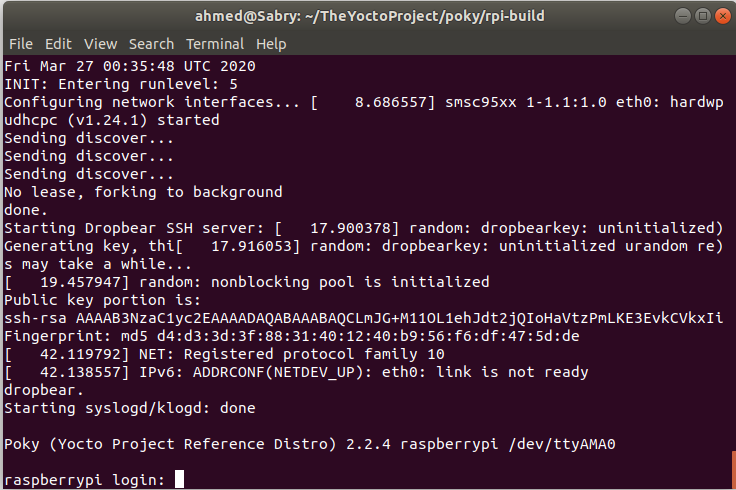
\includegraphics[scale=0.60]{./resources/img/boot-pi.png}
        \end{center}

      
      \end{itemize}
\end{enumerate}


\section{Appendix}
\subsection{Debugging the build messages}

\end{document}